% Created by tikzDevice version 0.10.1 on 2016-08-19 15:54:33
% !TEX encoding = UTF-8 Unicode
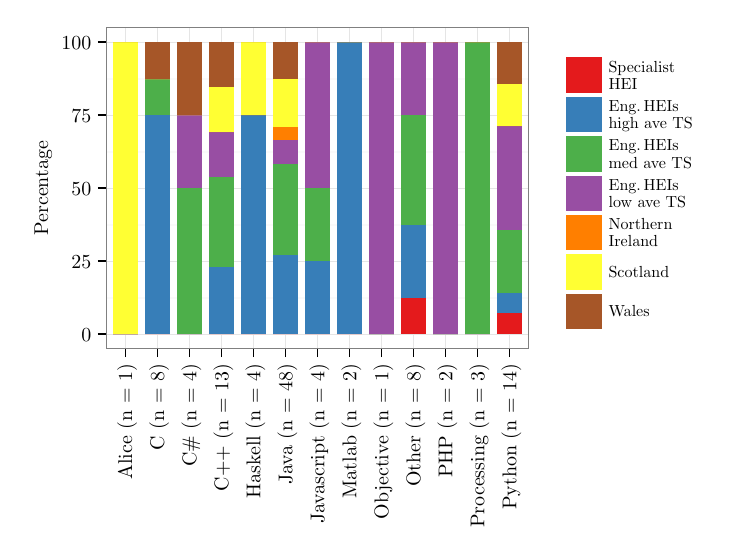
\begin{tikzpicture}[x=1pt,y=1pt]
\definecolor{fillColor}{RGB}{255,255,255}
\path[use as bounding box,fill=fillColor,fill opacity=0.00] (0,0) rectangle (252.94,180.67);
\begin{scope}
\path[clip] (  0.00,  0.00) rectangle (252.94,180.67);
\definecolor{drawColor}{RGB}{255,255,255}
\definecolor{fillColor}{RGB}{255,255,255}

\path[draw=drawColor,line width= 0.6pt,line join=round,line cap=round,fill=fillColor] (  0.00,  0.00) rectangle (252.94,180.68);
\end{scope}
\begin{scope}
\path[clip] ( 28.36, 64.59) rectangle (181.07,180.67);
\definecolor{fillColor}{RGB}{255,255,255}

\path[fill=fillColor] ( 28.36, 64.59) rectangle (181.07,180.68);
\definecolor{drawColor}{gray}{0.98}

\path[draw=drawColor,line width= 0.6pt,line join=round] ( 28.36, 83.05) --
	(181.07, 83.05);

\path[draw=drawColor,line width= 0.6pt,line join=round] ( 28.36,109.44) --
	(181.07,109.44);

\path[draw=drawColor,line width= 0.6pt,line join=round] ( 28.36,135.82) --
	(181.07,135.82);

\path[draw=drawColor,line width= 0.6pt,line join=round] ( 28.36,162.21) --
	(181.07,162.21);
\definecolor{drawColor}{gray}{0.90}

\path[draw=drawColor,line width= 0.2pt,line join=round] ( 28.36, 69.86) --
	(181.07, 69.86);

\path[draw=drawColor,line width= 0.2pt,line join=round] ( 28.36, 96.25) --
	(181.07, 96.25);

\path[draw=drawColor,line width= 0.2pt,line join=round] ( 28.36,122.63) --
	(181.07,122.63);

\path[draw=drawColor,line width= 0.2pt,line join=round] ( 28.36,149.01) --
	(181.07,149.01);

\path[draw=drawColor,line width= 0.2pt,line join=round] ( 28.36,175.40) --
	(181.07,175.40);

\path[draw=drawColor,line width= 0.2pt,line join=round] ( 35.30, 64.59) --
	( 35.30,180.67);

\path[draw=drawColor,line width= 0.2pt,line join=round] ( 46.87, 64.59) --
	( 46.87,180.67);

\path[draw=drawColor,line width= 0.2pt,line join=round] ( 58.44, 64.59) --
	( 58.44,180.67);

\path[draw=drawColor,line width= 0.2pt,line join=round] ( 70.01, 64.59) --
	( 70.01,180.67);

\path[draw=drawColor,line width= 0.2pt,line join=round] ( 81.58, 64.59) --
	( 81.58,180.67);

\path[draw=drawColor,line width= 0.2pt,line join=round] ( 93.14, 64.59) --
	( 93.14,180.67);

\path[draw=drawColor,line width= 0.2pt,line join=round] (104.71, 64.59) --
	(104.71,180.67);

\path[draw=drawColor,line width= 0.2pt,line join=round] (116.28, 64.59) --
	(116.28,180.67);

\path[draw=drawColor,line width= 0.2pt,line join=round] (127.85, 64.59) --
	(127.85,180.67);

\path[draw=drawColor,line width= 0.2pt,line join=round] (139.42, 64.59) --
	(139.42,180.67);

\path[draw=drawColor,line width= 0.2pt,line join=round] (150.99, 64.59) --
	(150.99,180.67);

\path[draw=drawColor,line width= 0.2pt,line join=round] (162.56, 64.59) --
	(162.56,180.67);

\path[draw=drawColor,line width= 0.2pt,line join=round] (174.13, 64.59) --
	(174.13,180.67);
\definecolor{fillColor}{RGB}{228,26,28}

\path[fill=fillColor] ( 30.67, 69.86) rectangle ( 39.93, 69.86);
\definecolor{fillColor}{RGB}{55,126,184}

\path[fill=fillColor] ( 30.67, 69.86) rectangle ( 39.93, 69.86);
\definecolor{fillColor}{RGB}{77,175,74}

\path[fill=fillColor] ( 30.67, 69.86) rectangle ( 39.93, 69.86);
\definecolor{fillColor}{RGB}{152,78,163}

\path[fill=fillColor] ( 30.67, 69.86) rectangle ( 39.93, 69.86);
\definecolor{fillColor}{RGB}{255,127,0}

\path[fill=fillColor] ( 30.67, 69.86) rectangle ( 39.93, 69.86);
\definecolor{fillColor}{RGB}{255,255,51}

\path[fill=fillColor] ( 30.67, 69.86) rectangle ( 39.93,175.40);
\definecolor{fillColor}{RGB}{166,86,40}

\path[fill=fillColor] ( 30.67,175.40) rectangle ( 39.93,175.40);
\definecolor{fillColor}{RGB}{228,26,28}

\path[fill=fillColor] ( 42.24, 69.86) rectangle ( 51.49, 69.86);
\definecolor{fillColor}{RGB}{55,126,184}

\path[fill=fillColor] ( 42.24, 69.86) rectangle ( 51.49,149.01);
\definecolor{fillColor}{RGB}{77,175,74}

\path[fill=fillColor] ( 42.24,149.01) rectangle ( 51.49,162.21);
\definecolor{fillColor}{RGB}{152,78,163}

\path[fill=fillColor] ( 42.24,162.21) rectangle ( 51.49,162.21);
\definecolor{fillColor}{RGB}{255,127,0}

\path[fill=fillColor] ( 42.24,162.21) rectangle ( 51.49,162.21);
\definecolor{fillColor}{RGB}{255,255,51}

\path[fill=fillColor] ( 42.24,162.21) rectangle ( 51.49,162.21);
\definecolor{fillColor}{RGB}{166,86,40}

\path[fill=fillColor] ( 42.24,162.21) rectangle ( 51.49,175.40);
\definecolor{fillColor}{RGB}{228,26,28}

\path[fill=fillColor] ( 53.81, 69.86) rectangle ( 63.06, 69.86);
\definecolor{fillColor}{RGB}{55,126,184}

\path[fill=fillColor] ( 53.81, 69.86) rectangle ( 63.06, 69.86);
\definecolor{fillColor}{RGB}{77,175,74}

\path[fill=fillColor] ( 53.81, 69.86) rectangle ( 63.06,122.63);
\definecolor{fillColor}{RGB}{152,78,163}

\path[fill=fillColor] ( 53.81,122.63) rectangle ( 63.06,149.01);
\definecolor{fillColor}{RGB}{255,127,0}

\path[fill=fillColor] ( 53.81,149.01) rectangle ( 63.06,149.01);
\definecolor{fillColor}{RGB}{255,255,51}

\path[fill=fillColor] ( 53.81,149.01) rectangle ( 63.06,149.01);
\definecolor{fillColor}{RGB}{166,86,40}

\path[fill=fillColor] ( 53.81,149.01) rectangle ( 63.06,175.40);
\definecolor{fillColor}{RGB}{228,26,28}

\path[fill=fillColor] ( 65.38, 69.86) rectangle ( 74.63, 69.86);
\definecolor{fillColor}{RGB}{55,126,184}

\path[fill=fillColor] ( 65.38, 69.86) rectangle ( 74.63, 94.22);
\definecolor{fillColor}{RGB}{77,175,74}

\path[fill=fillColor] ( 65.38, 94.22) rectangle ( 74.63,126.69);
\definecolor{fillColor}{RGB}{152,78,163}

\path[fill=fillColor] ( 65.38,126.69) rectangle ( 74.63,142.93);
\definecolor{fillColor}{RGB}{255,127,0}

\path[fill=fillColor] ( 65.38,142.93) rectangle ( 74.63,142.93);
\definecolor{fillColor}{RGB}{255,255,51}

\path[fill=fillColor] ( 65.38,142.93) rectangle ( 74.63,159.16);
\definecolor{fillColor}{RGB}{166,86,40}

\path[fill=fillColor] ( 65.38,159.16) rectangle ( 74.63,175.40);
\definecolor{fillColor}{RGB}{228,26,28}

\path[fill=fillColor] ( 76.95, 69.86) rectangle ( 86.20, 69.86);
\definecolor{fillColor}{RGB}{55,126,184}

\path[fill=fillColor] ( 76.95, 69.86) rectangle ( 86.20,149.01);
\definecolor{fillColor}{RGB}{77,175,74}

\path[fill=fillColor] ( 76.95,149.01) rectangle ( 86.20,149.01);
\definecolor{fillColor}{RGB}{152,78,163}

\path[fill=fillColor] ( 76.95,149.01) rectangle ( 86.20,149.01);
\definecolor{fillColor}{RGB}{255,127,0}

\path[fill=fillColor] ( 76.95,149.01) rectangle ( 86.20,149.01);
\definecolor{fillColor}{RGB}{255,255,51}

\path[fill=fillColor] ( 76.95,149.01) rectangle ( 86.20,175.40);
\definecolor{fillColor}{RGB}{166,86,40}

\path[fill=fillColor] ( 76.95,175.40) rectangle ( 86.20,175.40);
\definecolor{fillColor}{RGB}{228,26,28}

\path[fill=fillColor] ( 88.52, 69.86) rectangle ( 97.77, 69.86);
\definecolor{fillColor}{RGB}{55,126,184}

\path[fill=fillColor] ( 88.52, 69.86) rectangle ( 97.77, 98.45);
\definecolor{fillColor}{RGB}{77,175,74}

\path[fill=fillColor] ( 88.52, 98.45) rectangle ( 97.77,131.42);
\definecolor{fillColor}{RGB}{152,78,163}

\path[fill=fillColor] ( 88.52,131.42) rectangle ( 97.77,140.22);
\definecolor{fillColor}{RGB}{255,127,0}

\path[fill=fillColor] ( 88.52,140.22) rectangle ( 97.77,144.62);
\definecolor{fillColor}{RGB}{255,255,51}

\path[fill=fillColor] ( 88.52,144.62) rectangle ( 97.77,162.21);
\definecolor{fillColor}{RGB}{166,86,40}

\path[fill=fillColor] ( 88.52,162.21) rectangle ( 97.77,175.40);
\definecolor{fillColor}{RGB}{228,26,28}

\path[fill=fillColor] (100.09, 69.86) rectangle (109.34, 69.86);
\definecolor{fillColor}{RGB}{55,126,184}

\path[fill=fillColor] (100.09, 69.86) rectangle (109.34, 96.25);
\definecolor{fillColor}{RGB}{77,175,74}

\path[fill=fillColor] (100.09, 96.25) rectangle (109.34,122.63);
\definecolor{fillColor}{RGB}{152,78,163}

\path[fill=fillColor] (100.09,122.63) rectangle (109.34,175.40);
\definecolor{fillColor}{RGB}{255,127,0}

\path[fill=fillColor] (100.09,175.40) rectangle (109.34,175.40);
\definecolor{fillColor}{RGB}{255,255,51}

\path[fill=fillColor] (100.09,175.40) rectangle (109.34,175.40);
\definecolor{fillColor}{RGB}{166,86,40}

\path[fill=fillColor] (100.09,175.40) rectangle (109.34,175.40);
\definecolor{fillColor}{RGB}{228,26,28}

\path[fill=fillColor] (111.66, 69.86) rectangle (120.91, 69.86);
\definecolor{fillColor}{RGB}{55,126,184}

\path[fill=fillColor] (111.66, 69.86) rectangle (120.91,175.40);
\definecolor{fillColor}{RGB}{77,175,74}

\path[fill=fillColor] (111.66,175.40) rectangle (120.91,175.40);
\definecolor{fillColor}{RGB}{152,78,163}

\path[fill=fillColor] (111.66,175.40) rectangle (120.91,175.40);
\definecolor{fillColor}{RGB}{255,127,0}

\path[fill=fillColor] (111.66,175.40) rectangle (120.91,175.40);
\definecolor{fillColor}{RGB}{255,255,51}

\path[fill=fillColor] (111.66,175.40) rectangle (120.91,175.40);
\definecolor{fillColor}{RGB}{166,86,40}

\path[fill=fillColor] (111.66,175.40) rectangle (120.91,175.40);
\definecolor{fillColor}{RGB}{228,26,28}

\path[fill=fillColor] (123.22, 69.86) rectangle (132.48, 69.86);
\definecolor{fillColor}{RGB}{55,126,184}

\path[fill=fillColor] (123.22, 69.86) rectangle (132.48, 69.86);
\definecolor{fillColor}{RGB}{77,175,74}

\path[fill=fillColor] (123.22, 69.86) rectangle (132.48, 69.86);
\definecolor{fillColor}{RGB}{152,78,163}

\path[fill=fillColor] (123.22, 69.86) rectangle (132.48,175.40);
\definecolor{fillColor}{RGB}{255,127,0}

\path[fill=fillColor] (123.22,175.40) rectangle (132.48,175.40);
\definecolor{fillColor}{RGB}{255,255,51}

\path[fill=fillColor] (123.22,175.40) rectangle (132.48,175.40);
\definecolor{fillColor}{RGB}{166,86,40}

\path[fill=fillColor] (123.22,175.40) rectangle (132.48,175.40);
\definecolor{fillColor}{RGB}{228,26,28}

\path[fill=fillColor] (134.79, 69.86) rectangle (144.05, 83.05);
\definecolor{fillColor}{RGB}{55,126,184}

\path[fill=fillColor] (134.79, 83.05) rectangle (144.05,109.44);
\definecolor{fillColor}{RGB}{77,175,74}

\path[fill=fillColor] (134.79,109.44) rectangle (144.05,149.01);
\definecolor{fillColor}{RGB}{152,78,163}

\path[fill=fillColor] (134.79,149.01) rectangle (144.05,175.40);
\definecolor{fillColor}{RGB}{255,127,0}

\path[fill=fillColor] (134.79,175.40) rectangle (144.05,175.40);
\definecolor{fillColor}{RGB}{255,255,51}

\path[fill=fillColor] (134.79,175.40) rectangle (144.05,175.40);
\definecolor{fillColor}{RGB}{166,86,40}

\path[fill=fillColor] (134.79,175.40) rectangle (144.05,175.40);
\definecolor{fillColor}{RGB}{228,26,28}

\path[fill=fillColor] (146.36, 69.86) rectangle (155.62, 69.86);
\definecolor{fillColor}{RGB}{55,126,184}

\path[fill=fillColor] (146.36, 69.86) rectangle (155.62, 69.86);
\definecolor{fillColor}{RGB}{77,175,74}

\path[fill=fillColor] (146.36, 69.86) rectangle (155.62, 69.86);
\definecolor{fillColor}{RGB}{152,78,163}

\path[fill=fillColor] (146.36, 69.86) rectangle (155.62,175.40);
\definecolor{fillColor}{RGB}{255,127,0}

\path[fill=fillColor] (146.36,175.40) rectangle (155.62,175.40);
\definecolor{fillColor}{RGB}{255,255,51}

\path[fill=fillColor] (146.36,175.40) rectangle (155.62,175.40);
\definecolor{fillColor}{RGB}{166,86,40}

\path[fill=fillColor] (146.36,175.40) rectangle (155.62,175.40);
\definecolor{fillColor}{RGB}{228,26,28}

\path[fill=fillColor] (157.93, 69.86) rectangle (167.19, 69.86);
\definecolor{fillColor}{RGB}{55,126,184}

\path[fill=fillColor] (157.93, 69.86) rectangle (167.19, 69.86);
\definecolor{fillColor}{RGB}{77,175,74}

\path[fill=fillColor] (157.93, 69.86) rectangle (167.19,175.40);
\definecolor{fillColor}{RGB}{152,78,163}

\path[fill=fillColor] (157.93,175.40) rectangle (167.19,175.40);
\definecolor{fillColor}{RGB}{255,127,0}

\path[fill=fillColor] (157.93,175.40) rectangle (167.19,175.40);
\definecolor{fillColor}{RGB}{255,255,51}

\path[fill=fillColor] (157.93,175.40) rectangle (167.19,175.40);
\definecolor{fillColor}{RGB}{166,86,40}

\path[fill=fillColor] (157.93,175.40) rectangle (167.19,175.40);
\definecolor{fillColor}{RGB}{228,26,28}

\path[fill=fillColor] (169.50, 69.86) rectangle (178.76, 77.40);
\definecolor{fillColor}{RGB}{55,126,184}

\path[fill=fillColor] (169.50, 77.40) rectangle (178.76, 84.94);
\definecolor{fillColor}{RGB}{77,175,74}

\path[fill=fillColor] (169.50, 84.94) rectangle (178.76,107.55);
\definecolor{fillColor}{RGB}{152,78,163}

\path[fill=fillColor] (169.50,107.55) rectangle (178.76,145.25);
\definecolor{fillColor}{RGB}{255,127,0}

\path[fill=fillColor] (169.50,145.25) rectangle (178.76,145.25);
\definecolor{fillColor}{RGB}{255,255,51}

\path[fill=fillColor] (169.50,145.25) rectangle (178.76,160.32);
\definecolor{fillColor}{RGB}{166,86,40}

\path[fill=fillColor] (169.50,160.32) rectangle (178.76,175.40);
\definecolor{drawColor}{gray}{0.50}

\path[draw=drawColor,line width= 0.6pt,line join=round,line cap=round] ( 28.36, 64.59) rectangle (181.07,180.68);
\end{scope}
\begin{scope}
\path[clip] (  0.00,  0.00) rectangle (252.94,180.67);
\definecolor{drawColor}{RGB}{0,0,0}

\node[text=drawColor,anchor=base east,inner sep=0pt, outer sep=0pt, scale=  0.72] at ( 22.96, 67.38) {0};

\node[text=drawColor,anchor=base east,inner sep=0pt, outer sep=0pt, scale=  0.72] at ( 22.96, 93.77) {25};

\node[text=drawColor,anchor=base east,inner sep=0pt, outer sep=0pt, scale=  0.72] at ( 22.96,120.15) {50};

\node[text=drawColor,anchor=base east,inner sep=0pt, outer sep=0pt, scale=  0.72] at ( 22.96,146.53) {75};

\node[text=drawColor,anchor=base east,inner sep=0pt, outer sep=0pt, scale=  0.72] at ( 22.96,172.92) {100};
\end{scope}
\begin{scope}
\path[clip] (  0.00,  0.00) rectangle (252.94,180.67);
\definecolor{drawColor}{RGB}{0,0,0}

\path[draw=drawColor,line width= 0.6pt,line join=round] ( 25.36, 69.86) --
	( 28.36, 69.86);

\path[draw=drawColor,line width= 0.6pt,line join=round] ( 25.36, 96.25) --
	( 28.36, 96.25);

\path[draw=drawColor,line width= 0.6pt,line join=round] ( 25.36,122.63) --
	( 28.36,122.63);

\path[draw=drawColor,line width= 0.6pt,line join=round] ( 25.36,149.01) --
	( 28.36,149.01);

\path[draw=drawColor,line width= 0.6pt,line join=round] ( 25.36,175.40) --
	( 28.36,175.40);
\end{scope}
\begin{scope}
\path[clip] (  0.00,  0.00) rectangle (252.94,180.67);
\definecolor{drawColor}{RGB}{0,0,0}

\path[draw=drawColor,line width= 0.6pt,line join=round] ( 35.30, 61.59) --
	( 35.30, 64.59);

\path[draw=drawColor,line width= 0.6pt,line join=round] ( 46.87, 61.59) --
	( 46.87, 64.59);

\path[draw=drawColor,line width= 0.6pt,line join=round] ( 58.44, 61.59) --
	( 58.44, 64.59);

\path[draw=drawColor,line width= 0.6pt,line join=round] ( 70.01, 61.59) --
	( 70.01, 64.59);

\path[draw=drawColor,line width= 0.6pt,line join=round] ( 81.58, 61.59) --
	( 81.58, 64.59);

\path[draw=drawColor,line width= 0.6pt,line join=round] ( 93.14, 61.59) --
	( 93.14, 64.59);

\path[draw=drawColor,line width= 0.6pt,line join=round] (104.71, 61.59) --
	(104.71, 64.59);

\path[draw=drawColor,line width= 0.6pt,line join=round] (116.28, 61.59) --
	(116.28, 64.59);

\path[draw=drawColor,line width= 0.6pt,line join=round] (127.85, 61.59) --
	(127.85, 64.59);

\path[draw=drawColor,line width= 0.6pt,line join=round] (139.42, 61.59) --
	(139.42, 64.59);

\path[draw=drawColor,line width= 0.6pt,line join=round] (150.99, 61.59) --
	(150.99, 64.59);

\path[draw=drawColor,line width= 0.6pt,line join=round] (162.56, 61.59) --
	(162.56, 64.59);

\path[draw=drawColor,line width= 0.6pt,line join=round] (174.13, 61.59) --
	(174.13, 64.59);
\end{scope}
\begin{scope}
\path[clip] (  0.00,  0.00) rectangle (252.94,180.67);
\definecolor{drawColor}{RGB}{0,0,0}

\node[text=drawColor,rotate= 90.00,anchor=base east,inner sep=0pt, outer sep=0pt, scale=  0.72] at ( 37.78, 59.19) {Alice (n = 1)};

\node[text=drawColor,rotate= 90.00,anchor=base east,inner sep=0pt, outer sep=0pt, scale=  0.72] at ( 49.35, 59.19) {C (n = 8)};

\node[text=drawColor,rotate= 90.00,anchor=base east,inner sep=0pt, outer sep=0pt, scale=  0.72] at ( 60.92, 59.19) {C\# (n = 4)};

\node[text=drawColor,rotate= 90.00,anchor=base east,inner sep=0pt, outer sep=0pt, scale=  0.72] at ( 72.49, 59.19) {C++ (n = 13)};

\node[text=drawColor,rotate= 90.00,anchor=base east,inner sep=0pt, outer sep=0pt, scale=  0.72] at ( 84.05, 59.19) {Haskell (n = 4)};

\node[text=drawColor,rotate= 90.00,anchor=base east,inner sep=0pt, outer sep=0pt, scale=  0.72] at ( 95.62, 59.19) {Java (n = 48)};

\node[text=drawColor,rotate= 90.00,anchor=base east,inner sep=0pt, outer sep=0pt, scale=  0.72] at (107.19, 59.19) {Javascript (n = 4)};

\node[text=drawColor,rotate= 90.00,anchor=base east,inner sep=0pt, outer sep=0pt, scale=  0.72] at (118.76, 59.19) {Matlab (n = 2)};

\node[text=drawColor,rotate= 90.00,anchor=base east,inner sep=0pt, outer sep=0pt, scale=  0.72] at (130.33, 59.19) {Objective (n = 1)};

\node[text=drawColor,rotate= 90.00,anchor=base east,inner sep=0pt, outer sep=0pt, scale=  0.72] at (141.90, 59.19) {Other (n = 8)};

\node[text=drawColor,rotate= 90.00,anchor=base east,inner sep=0pt, outer sep=0pt, scale=  0.72] at (153.47, 59.19) {PHP (n = 2)};

\node[text=drawColor,rotate= 90.00,anchor=base east,inner sep=0pt, outer sep=0pt, scale=  0.72] at (165.04, 59.19) {Processing (n = 3)};

\node[text=drawColor,rotate= 90.00,anchor=base east,inner sep=0pt, outer sep=0pt, scale=  0.72] at (176.61, 59.19) {Python (n = 14)};
\end{scope}
\begin{scope}
\path[clip] (  0.00,  0.00) rectangle (252.94,180.67);
\definecolor{drawColor}{RGB}{0,0,0}

\node[text=drawColor,rotate= 90.00,anchor=base,inner sep=0pt, outer sep=0pt, scale=  0.72] at (  7.36,122.63) {Percentage};
\end{scope}
\begin{scope}
\path[clip] (  0.00,  0.00) rectangle (252.94,180.67);
\definecolor{fillColor}{RGB}{255,255,255}

\path[fill=fillColor] (189.61, 66.76) rectangle (244.41,178.50);
\end{scope}
\begin{scope}
\path[clip] (  0.00,  0.00) rectangle (252.94,180.67);
\definecolor{fillColor}{RGB}{228,26,28}

\path[fill=fillColor] (194.59,157.10) rectangle (207.39,169.90);
\end{scope}
\begin{scope}
\path[clip] (  0.00,  0.00) rectangle (252.94,180.67);
\definecolor{fillColor}{RGB}{55,126,184}

\path[fill=fillColor] (194.59,142.87) rectangle (207.39,155.68);
\end{scope}
\begin{scope}
\path[clip] (  0.00,  0.00) rectangle (252.94,180.67);
\definecolor{fillColor}{RGB}{77,175,74}

\path[fill=fillColor] (194.59,128.65) rectangle (207.39,141.45);
\end{scope}
\begin{scope}
\path[clip] (  0.00,  0.00) rectangle (252.94,180.67);
\definecolor{fillColor}{RGB}{152,78,163}

\path[fill=fillColor] (194.59,114.42) rectangle (207.39,127.23);
\end{scope}
\begin{scope}
\path[clip] (  0.00,  0.00) rectangle (252.94,180.67);
\definecolor{fillColor}{RGB}{255,127,0}

\path[fill=fillColor] (194.59,100.20) rectangle (207.39,113.00);
\end{scope}
\begin{scope}
\path[clip] (  0.00,  0.00) rectangle (252.94,180.67);
\definecolor{fillColor}{RGB}{255,255,51}

\path[fill=fillColor] (194.59, 85.97) rectangle (207.39, 98.77);
\end{scope}
\begin{scope}
\path[clip] (  0.00,  0.00) rectangle (252.94,180.67);
\definecolor{fillColor}{RGB}{166,86,40}

\path[fill=fillColor] (194.59, 71.74) rectangle (207.39, 84.55);
\end{scope}
\begin{scope}
\path[clip] (  0.00,  0.00) rectangle (252.94,180.67);
\definecolor{drawColor}{RGB}{0,0,0}

\node[text=drawColor,anchor=base west,inner sep=0pt, outer sep=0pt, scale=  0.58] at (209.91,164.63) {Specialist};

\node[text=drawColor,anchor=base west,inner sep=0pt, outer sep=0pt, scale=  0.58] at (209.91,158.41) {HEI};
\end{scope}
\begin{scope}
\path[clip] (  0.00,  0.00) rectangle (252.94,180.67);
\definecolor{drawColor}{RGB}{0,0,0}

\node[text=drawColor,anchor=base west,inner sep=0pt, outer sep=0pt, scale=  0.58] at (209.91,150.40) {Eng.\,HEIs};

\node[text=drawColor,anchor=base west,inner sep=0pt, outer sep=0pt, scale=  0.58] at (209.91,144.18) {high ave TS};
\end{scope}
\begin{scope}
\path[clip] (  0.00,  0.00) rectangle (252.94,180.67);
\definecolor{drawColor}{RGB}{0,0,0}

\node[text=drawColor,anchor=base west,inner sep=0pt, outer sep=0pt, scale=  0.58] at (209.91,136.18) {Eng.\,HEIs};

\node[text=drawColor,anchor=base west,inner sep=0pt, outer sep=0pt, scale=  0.58] at (209.91,129.96) {med ave TS};
\end{scope}
\begin{scope}
\path[clip] (  0.00,  0.00) rectangle (252.94,180.67);
\definecolor{drawColor}{RGB}{0,0,0}

\node[text=drawColor,anchor=base west,inner sep=0pt, outer sep=0pt, scale=  0.58] at (209.91,121.95) {Eng.\,HEIs};

\node[text=drawColor,anchor=base west,inner sep=0pt, outer sep=0pt, scale=  0.58] at (209.91,115.73) {low ave TS};
\end{scope}
\begin{scope}
\path[clip] (  0.00,  0.00) rectangle (252.94,180.67);
\definecolor{drawColor}{RGB}{0,0,0}

\node[text=drawColor,anchor=base west,inner sep=0pt, outer sep=0pt, scale=  0.58] at (209.91,107.72) {Northern};

\node[text=drawColor,anchor=base west,inner sep=0pt, outer sep=0pt, scale=  0.58] at (209.91,101.50) {Ireland};
\end{scope}
\begin{scope}
\path[clip] (  0.00,  0.00) rectangle (252.94,180.67);
\definecolor{drawColor}{RGB}{0,0,0}

\node[text=drawColor,anchor=base west,inner sep=0pt, outer sep=0pt, scale=  0.58] at (209.91, 90.39) {Scotland};
\end{scope}
\begin{scope}
\path[clip] (  0.00,  0.00) rectangle (252.94,180.67);
\definecolor{drawColor}{RGB}{0,0,0}

\node[text=drawColor,anchor=base west,inner sep=0pt, outer sep=0pt, scale=  0.58] at (209.91, 76.16) {Wales};
\end{scope}
\end{tikzpicture}
